\documentclass{article}
\usepackage[T2A]{fontenc}
\usepackage[utf8]{inputenc}
\usepackage[russian]{babel}
\usepackage{amssymb,amsmath,amsthm}
\usepackage{systeme,mathtools}
\usepackage{lipsum}
\usepackage{relsize}
\newcommand\md{\ }
\usepackage[normalem]{ulem}
\usepackage{pdfpages}

\begin{document}
\selectlanguage{russian}

\includepdf[pages=-]{Ok.pdf}
\section{Задание}

1. Создать проект в IntelliJ IDEA

2. Cоздать собственный Git репозитарий

3. Написать программу, в результате которой считается сумма элементов целочисленного массива с помощью циклов for, while, do while, результат выводится на экран.

4. Написать программу, в результате которой выводятся на экран аргументы командной строки в цикле for.

5. Написать программу, в результате работы которой выводятся на экран первые 10 чисел гармонического ряда (форматировать вывод).

6. Написать программу, в результате которой генерируется массив целых чисел случайным образом, вывести его на экран, отсортировать его, и снова вывести на экран (использовать два подхода к генерации случайных чисел – метод random() класса Math и класс Random).

7. Написать программу, которая с помощью метода, вычисляет факториал числа (использовать управляющую конструкцию цикла), проверить работу метода.

8. Результаты выполнения практической работы залить через IDE в свой репозитарий и продемонстрировать преподавателю.

\section{Ход работы}

В ходе выполнения работы были получены следующие исходные коды:

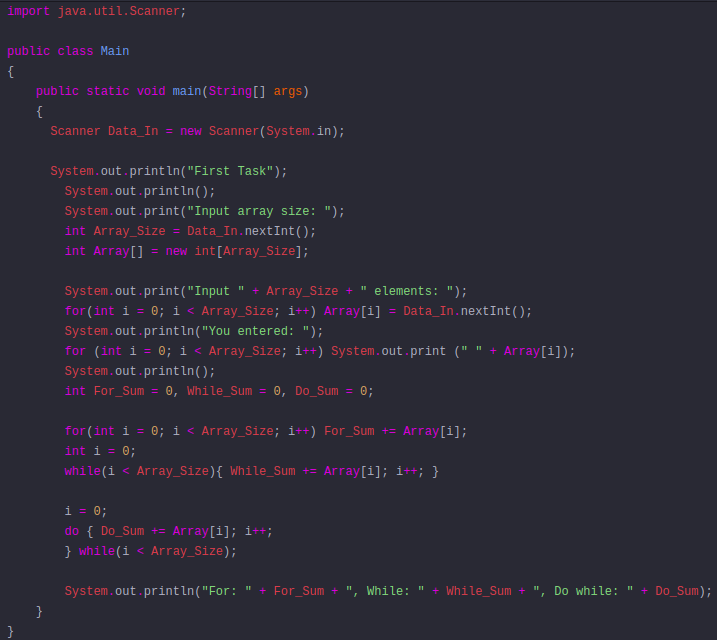
\includegraphics[width=0.7\linewidth]{view1.png}

\caption{Рисунок 1. Фрагмент кода для реализации задания с массивами.}

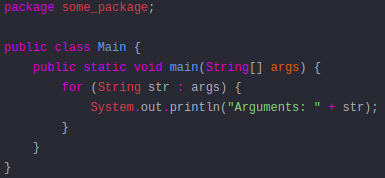
\includegraphics[width=0.9\linewidth]{view2.png}

\caption{Рисунок 2. Фрагмент кода для реализации задания с командной строкой.}

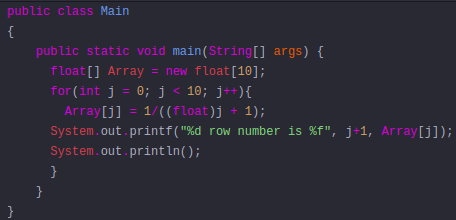
\includegraphics[width=0.9\linewidth]{view3.png}

\caption{Рисунок 3. Фрагмент кода для реализации задания с форматированием.}

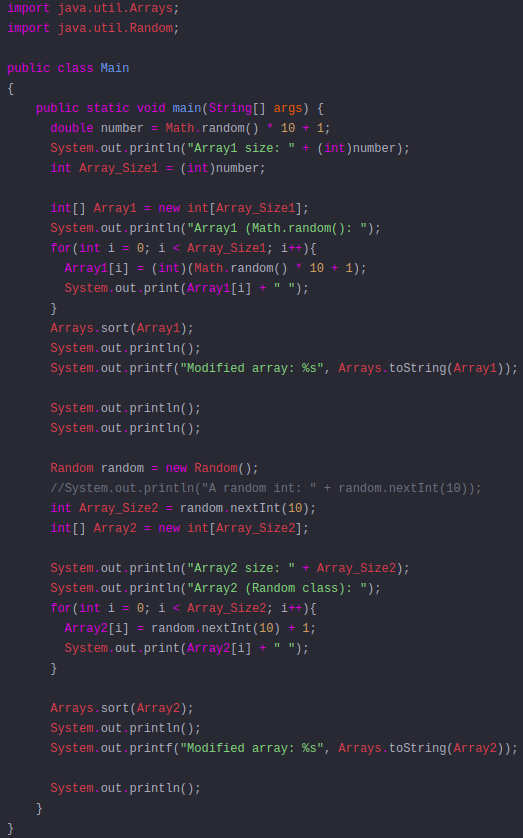
\includegraphics[width=0.9\linewidth]{view4.png}

\caption{Рисунок 4. Фрагмент кода для реализации задания со случайными числами.}

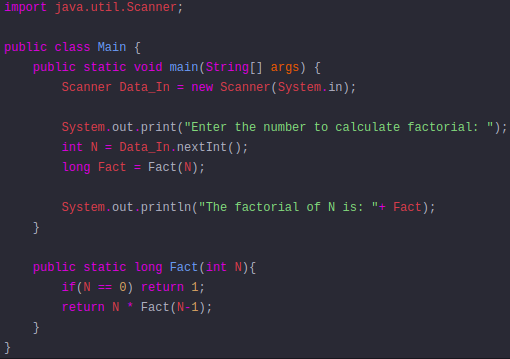
\includegraphics[width=0.7\linewidth]{view5.png}

\caption{Рисунок 5. Фрагмент кода для реализации задания с факториалом.}

\section{Вывод}
В ходе выполнения практического занятия номер 1 я научилась решать задачи счета суммы элементов целочисленного массива с помощью циклов, вывода на экран аргументов командной строки в цикле и первых 10 чисел гармонического ряда с форматированием вывода с помощью написания программа на языке Java. Также были написаны программы для решения задач генерирования массива целых чисел случайным образом, вычисления факториала числа.

\end{document}
